%!TEX root = ../main.tex
\section{Kết quả thực nghiệm}

\subsection{10 tác vụ}
    \begin{frame}{Dữ liệu thử nghiệm và cài đặt các thuật toán}
        \begin{block}{Mô tả bộ dữ liệu MaTO-10}
            \begin{itemize}
                \item Bộ MaTO-10 \footfullcite{chen2019adaptive} gồm $10$ tác vụ tương ứng với $10$ hàm số thực $25$ hoặc $50$ biến.
                \item $T_1, \ldots, T_4$ dễ, $T_6, \ldots, T_{10}$ khó.
                \item Biết trước $T_1$ hỗ trợ $T_5$, $T_2$ hỗ trợ $T_6$, $T_3, T_4$ hỗ trợ $T_7$, $T_4$ hỗ trợ $T_9$.
                \item Phục vụ phân tích mô đun ghép cặp các tác vụ hoạt động đúng hay không.
            \end{itemize}
        \end{block}
        \begin{columns}
            \begin{column}{0.48\textwidth}
                \begin{exampleblock}{Tham số của MFEA/EBSGA/\gls{propose}}
                    \begin{itemize}
                        \item Kích thước quần thể: 100
                        \item rmp: 0.3
                        \item sbxdi: 2
                        \item pmdi: 5
                    \end{itemize}
                \end{exampleblock}
            \end{column}
            \begin{column}{0.48\textwidth}
                \begin{exampleblock}{Tham số của MaTGA}
                    Dùng tham số mặc định của tác giả ${ }^{a}$
                \end{exampleblock}
            \end{column}
        \end{columns}
    \end{frame}

    \begin{frame}{Kết quả tối ưu}
        \begin{table}[H]
            \begin{tabular}{@{}ccccc@{}}
                \toprule
                \textbf{Task} & \gls{propose} & MFEA & MaTGA & EBSGA \\ \midrule
                $T_1$ & \textbf{3.72E-05}   & 1.31E+00 $(-)$          & 2.45E-04          $(-)$ & 5.58E-04 $(-)$ \\
                $T_2$ & \textbf{6.48E-06}   & 1.27E+00 $(-)$          & 4.75E-04          $(-)$ & 6.10E-05 $(-)$ \\
                $T_3$ & \textbf{4.35E-07}   & 1.17E+00 $(-)$          & \textbf{0.00E+00} $(\approx)$ & 2.00E-06 $(-)$ \\
                $T_4$ & \textbf{7.09E-13}   & 3.37E+00 $(-)$          & 1.00E-06          $(-)$ & 1.60E-05 $(-)$ \\
                $T_5$ & 1.74E+01            & 8.15E+02 $(-)$          & \textbf{2.16E-02} $(+)$ & 3.29E-02 $(+)$ \\
                $T_6$ & \textbf{7.03E-04}   & 1.99E+01 $(-)$          & 3.61E-03          $(-)$ & \textbf{8.59E-04} $(\approx)$ \\
                $T_7$ & 1.00E-02            & 1.05E+01 $(-)$          & \textbf{5.57E-04} $(+)$ & 1.60E-03 $(+)$ \\
                $T_8$ & 1.89E+02            & 2.34E+03 $(-)$          & \textbf{3.40E-02} $(-)$ & 4.73E-02 $(-)$ \\
                $T_9$ & \textbf{4.00E-07}   & 4.11E+02 $(-)$          & 4.52E-03          $(-)$ & 4.58E-03 $(-)$ \\
                $T_{10}$ & 2.74E+01            & \textbf{1.54E+01} $(+)$ & 1.57E+01          $(+)$ & 3.41E+01 $(-)$ \\
                \bottomrule
            \end{tabular}
            \caption{Giá trị trung bình hàm mục tiêu của các thuật toán tiến hóa đa nhiệm sau 30 lần chạy độc lập. $(-, +, and \approx$ thể hiện thuật toán kém đáng kể, tốt đáng kể hoặc tương đương với \gls{propose}, kiểm định bằng Wilcoxon signed-rank test $\alpha=0.05)$}
            \label{tab:experiment:last10}
        \end{table}
    \end{frame}
    \begin{frame}{Kết quả ghép cặp}
        \begin{figure}
            \centering
            \begin{subfigure}[b]{0.245\linewidth}
                \centering
                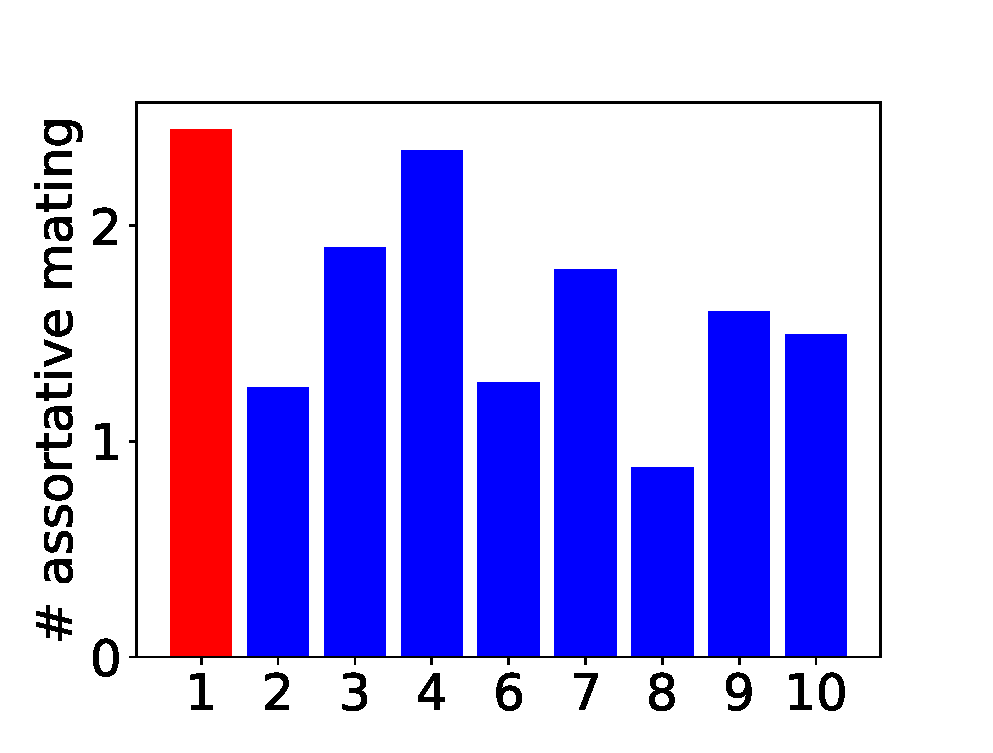
\includegraphics[width=\linewidth]{figure/experiment/bar10/5.eps}
                \caption{Tác vụ 5}
                \label{fig:bar10-5}
            \end{subfigure}
            \hfill
            \begin{subfigure}[b]{0.245\linewidth}
                \centering
                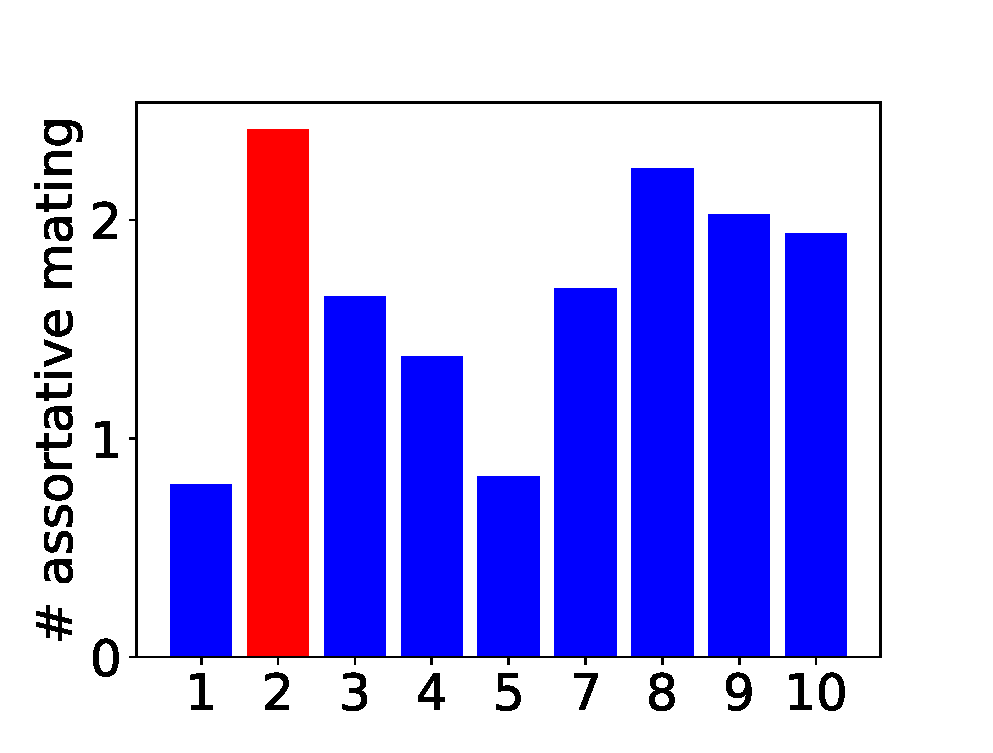
\includegraphics[width=\linewidth]{figure/experiment/bar10/6.eps}
                \caption{Tác vụ 6}
                \label{fig:bar10-6}
            \end{subfigure}
            \hfill
            \begin{subfigure}[b]{0.245\linewidth}
                \centering
                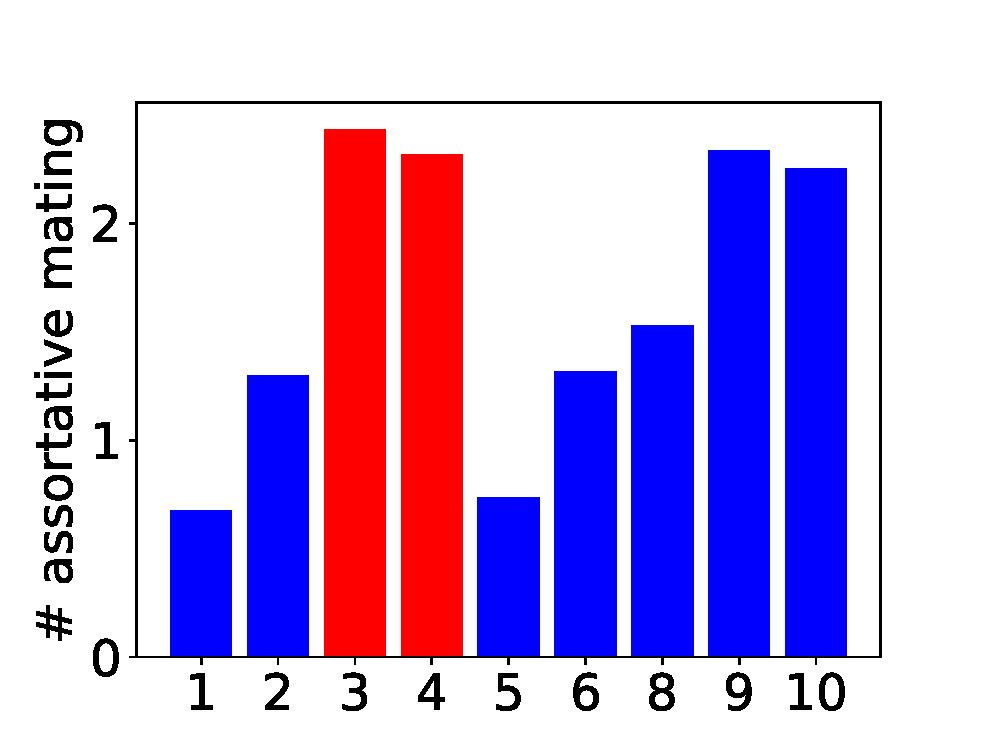
\includegraphics[width=\linewidth]{figure/experiment/bar10/7.eps}
                \caption{Tác vụ 7}
                \label{fig:bar10-7}
            \end{subfigure}
            \hfill
            \begin{subfigure}[b]{0.245\linewidth}
                \centering
                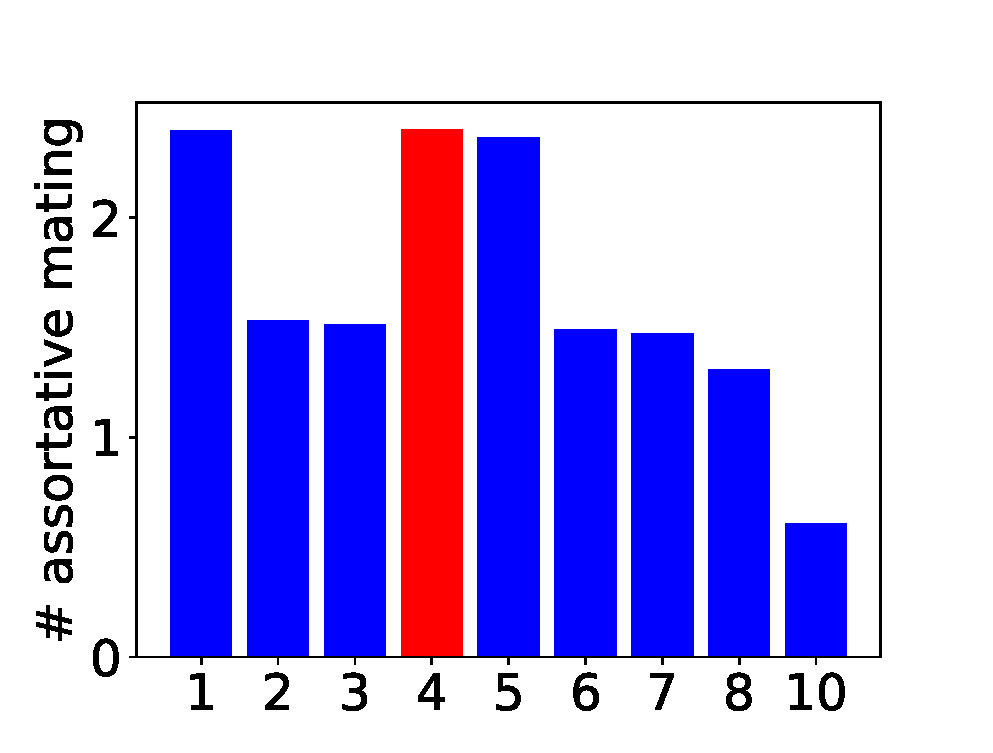
\includegraphics[width=\linewidth]{figure/experiment/bar10/9.eps}
                \caption{Tác vụ 9}
                \label{fig:bar10-9}
            \end{subfigure}
            \hfill
            \caption{Số lần trung bình mỗi thế hệ mỗi tác vụ chọn ghép cặp với tác vụ khác trong \gls{propose}. Tác vụ hỗ trợ thật được hiển thị bằng màu đỏ.}
            \label{fig:result:count10}
        \end{figure}
    \end{frame}

\subsection{50 tác vụ}
    \begin{frame}{Dữ liệu thử nghiệm}
        \begin{block}{Mô tả bộ dữ liệu MaTO-50}
            \begin{itemize}
                \item $10$ bộ, mỗi bộ $50$ tác vụ tương ứng với $50$ hàm số thực $50$ biến.
                \item Không biết trước mối quan hệ giữa các hàm.
                \item Đa dạng hơn MaTO-10.
                \item Cuộc thi của hội thảo WCCI/GECCO 2020.
            \end{itemize}
        \end{block}
    \end{frame}
    \begin{frame}{Kết quả tối ưu}
        \begin{table}[hp]
            \centering
            \begin{tabular}{@{}ccccc@{}}
                \toprule
                \textbf{Benchmark} & \gls{propose} & MFEA & MaTGA & EBSGA \\ \midrule
                $B_1$    & \textbf{50 (50)} & 0 (0) & 0 (0)           & 0 (0) \\
                $B_2$    & \textbf{50 (50)} & 0 (0) & 0 (0)           & 0 (0) \\
                $B_3$    & 8 (0)            & 0 (0) & \textbf{42 (8)} & 0 (0) \\
                $B_4$    & 17 (9)           & 0 (0) & 0 (0)           & \textbf{33 (33)} \\
                $B_5$    & \textbf{50 (50)} & 0 (0) & 0 (0)           & 0 (0) \\
                $B_6$    & \textbf{50 (50)} & 0 (0) & 0 (0)           & 0 (0) \\
                $B_7$    & 3 (0)            & 0 (0) & 14 (2)          & \textbf{33 (28)} \\
                $B_8$    & \textbf{30 (28)} & 0 (0) & 0 (0)           & 20 (20) \\
                $B_9$    & \textbf{42 (42)} & 0 (0) & 0 (0)           & 8 (8) \\
                $B_{10}$ & 8 (6)            & 2 (0) & 11 (10)         & \textbf{29 (23)} \\
                \bottomrule
            \end{tabular}
            \caption{Bảng thể hiện số lần một thuật toán giải tốt nhất và tốt nhất đáng kể trên $10$ tập hàm đánh giá, mỗi tập có $50$ hàm đánh giá của bộ dữ liệu MaTO-50, thống kê lại sau $30$ lần chạy độc lập.}
            \label{tab:experiment:last10}
        \end{table}
    \end{frame}
    \begin{frame}{So sánh thời gian chạy}
        \begin{figure}[H]
            \centering
            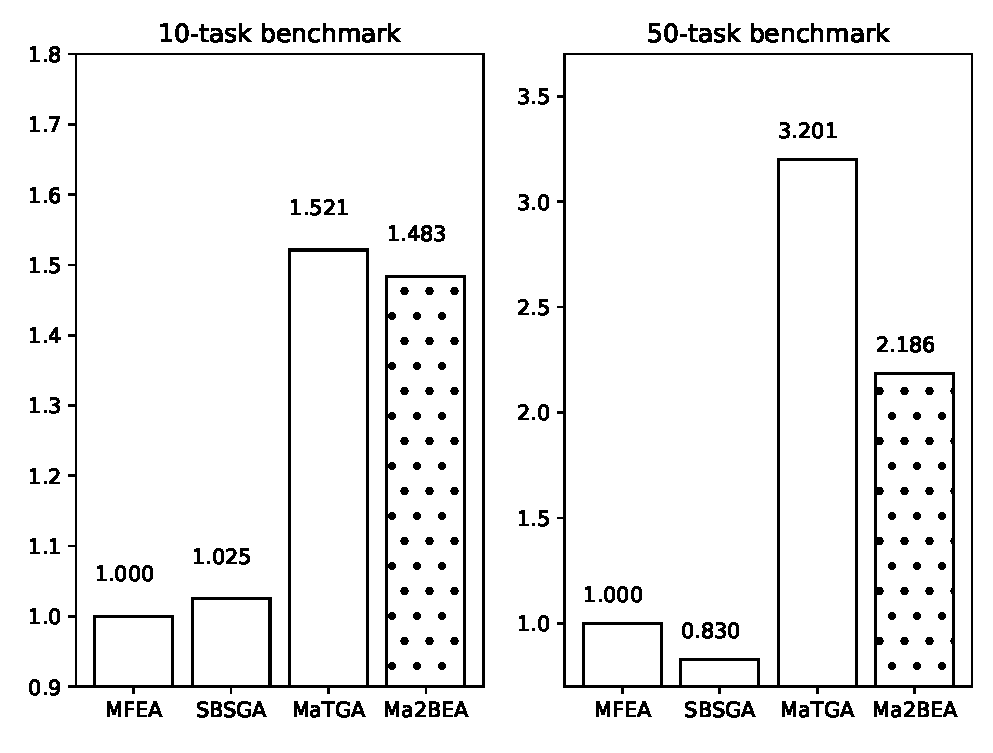
\includegraphics[width=0.7\linewidth]{figure/experiment/runtime.eps}
            \caption{Thời gian chạy của các thuật toán tiến hóa đa nhiệm, lấy thời gian chạy của \gls{mfea} trên cũng một một trường thực nghiệm, cùng ngôn ngữ lập trình làm chuẩn}
            \label{fig:experiment:runtime}
        \end{figure}
    \end{frame}

\subsection{Mujoco Multitask}
    \begin{frame}{Dữ liệu thử nghiệm}
        \begin{block}{Dữ liệu thử nghiệm}
            \begin{itemize}
                \item Sử dụng bộ Mujoco Multitask \footfullcite{henderson2018deep}.
                \item Thực nghiệm trên hai tập dữ liệu \emph{Hopper-gravity} và \emph{Hopper-size}
            \end{itemize}
            \begin{figure}
                \centering
                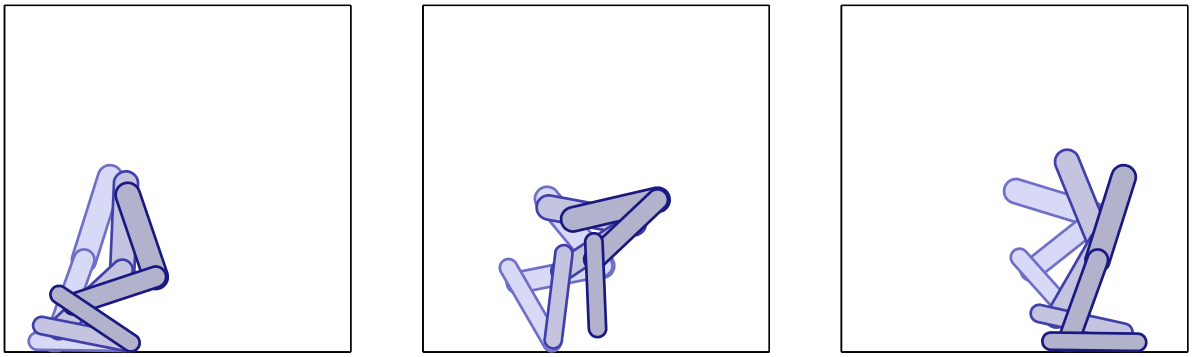
\includegraphics[width=0.8\linewidth]{figure/experiment/hopper.png}
                \caption{Minh họa cách hoạt động của robot Hopper \cite{erez2011infinite}.}
                \label{fig:result:benchmark:hopper}
            \end{figure}
        \end{block}
    \end{frame}

    \begin{frame}{Cài đặt thực nghiệm}
        \begin{columns}
            \begin{column}{0.48\textwidth}
                \begin{block}{Môi trường}
                    \begin{itemize}
                        \item \textbf{Trạng thái:} $s \in \mathbb{R}^{11}$
                        \item \textbf{Hành động:} $a \in \mathbb{R}^{3}$
                    \end{itemize}
                \end{block}
            \end{column}
            \begin{column}{0.48\textwidth}
                \begin{block}{Mô hình ra quyết định cần tối ưu}
                    \begin{itemize}
                        \item \textbf{Đầu vào: } là $11$ chiều
                        \item \textbf{Lớp ẩn: } chứa $16$ nút
                        \item \textbf{Activation: } tanh
                        \item \textbf{Đầu ra: } là $3$ chiều
                        \item \textbf{Không gian biểu diễn chung:} $[0, 1] ^ {243}$.
                        \item \textbf{Giải mã: } dãn từ khoảng $[0, 1]$ đến $[-5, 5]$.
                        \item $(T, N) = (100, 10)$
                    \end{itemize}
                \end{block}
            \end{column}
        \end{columns}
    \end{frame}

    \begin{frame}{Kết quả tối ưu}
        \begin{figure}[hp]
            \centering
            \begin{subfigure}[b]{0.49\linewidth}
                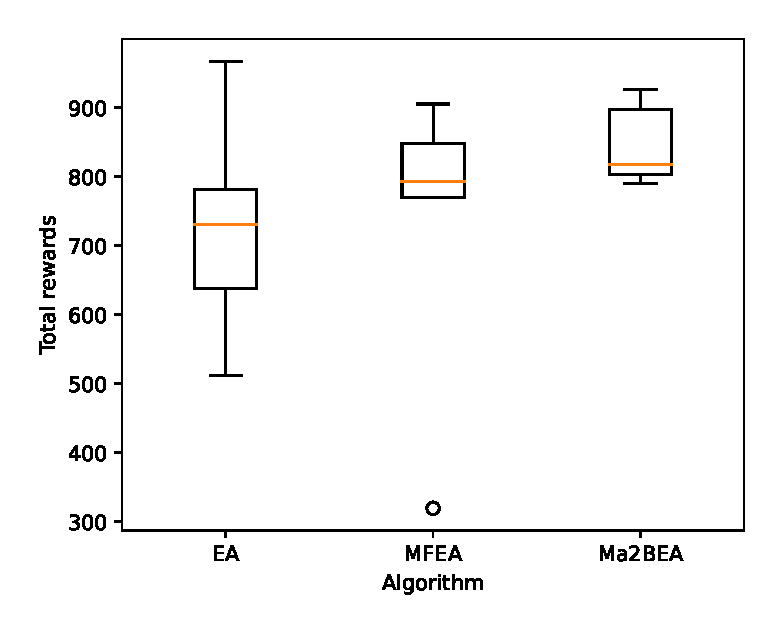
\includegraphics[width=\linewidth]{figure/experiment/mujoco/hopper-gravity.eps}
                \caption{$Hopper-gravity$}
                \label{fig:result:mujoco:sphere}
            \end{subfigure}
            \hfill
            \begin{subfigure}[b]{0.49\linewidth}
                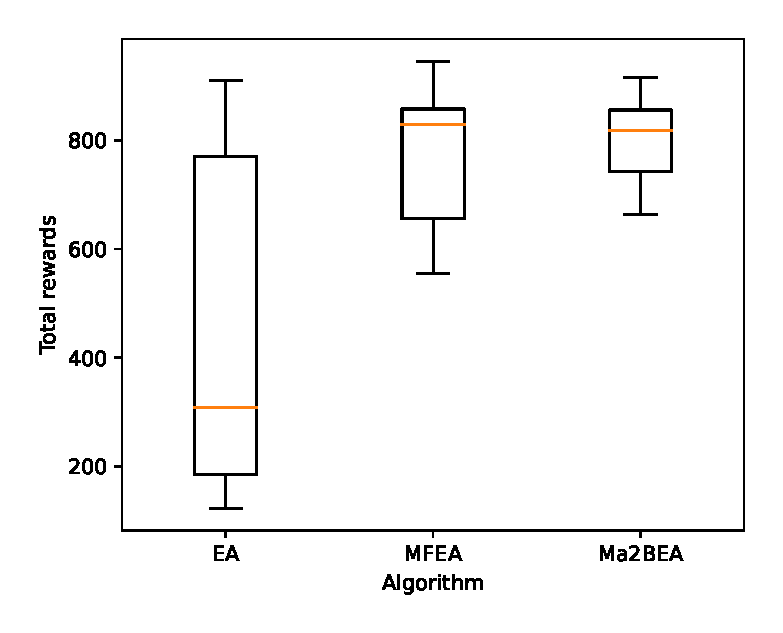
\includegraphics[width=\linewidth]{figure/experiment/mujoco/hopper-size.eps}
                \caption{$Hopper-size$}
                \label{fig:result:mujoco:weierstrass}
            \end{subfigure}
            \hfill
            \caption{Biểu đồ hộp (minh hoạ các giá trị nhỏ nhất, quartile thứ nhất, median, quartile thứ ba, giá trị lớn nhất) của các hàm mục tiêu của bộ Mujoco Multitask, giải bởi \gls{ea}, \gls{mfea}, và \gls{propose}.
                     Giá trị được thống kê ở biểu đồ hộp là giá trị hàm mục tiêu tại thế hệ cuối cùng của các tác vụ khác nhau, giải bởi từng thuật toán trên từng bộ dữ liệu.}
            \label{fig:result:mujoco}
        \end{figure}
    \end{frame}
    
